%%%%%%%%%%%%%%%%%%%%%%%%%%%%%%%%%%%%%%%%%%%%%%%%%%%%%%%%%%%%%%%%%%%%%
%%%
%%% Set these variables appropriately
%%%
\newcommand{\AUTHORS}{Jenny Louthan \date{\today}}
\newcommand{\TITLE}{irpSSHa: Identifying and Reporting Potential SSH Attackers from IP Flow Logs}
\newcommand{\KEYWORDS}{}
\newcommand{\CONFERENCE}{}
\newcommand{\PAGENUMBERS}{yes}       % "yes" or "no"
\newcommand{\TOAPPEAR}{no}
%%%
%%%
%%%%%%%%%%%%%%%%%%%%%%%%%%%%%%%%%%%%%%%%%%%%%%%%%%%%%%%%%%%%%%%%%%%%%

%%%% Setup the document/page
\documentclass[pdftex,twoside,twocolumn,11pt,letterpaper]{article}
\usepackage{ifthen}
\usepackage{listings}

\ifthenelse{\equal{\PAGENUMBERS}{yes}}{%
\usepackage[nohead,
            left=1in,right=1in,top=1in,
            footskip=0.5in,bottom=0.75in     % Room for page numbers
            ]{geometry}
}{%
\usepackage[noheadfoot,columnsep=0.2in,
            margin=1in,centering,truedimen]{geometry}
}

\usepackage{fancyhdr}
\usepackage[numbers,sort]{natbib}
\usepackage{xspace}
\usepackage{booktabs}
\usepackage{subfigure}
\usepackage[T1]{fontenc}
\usepackage{textcomp}
\usepackage{mathptmx}   % Times + Times-like math symbols
\usepackage{courier}
\usepackage[scaled=0.92]{helvet}

\usepackage{color}
\usepackage[pdftex]{graphicx}
\ifthenelse{\isundefined{\wantBW}}{%
  \usepackage[colorlinks]{hyperref}%        % for online version
}{%
  \usepackage[pdfborder={0 0 0}]{hyperref}% % for paper (B&W) version
}
\newcommand{\URL}[1]{\url{#1}}

%%%%% Setup for PDF
\hypersetup{%
pdfauthor = {\AUTHORS},
pdftitle = {\TITLE},
pdfsubject = {\CONFERENCE},
pdfkeywords = {\KEYWORDS},
bookmarksopen = {true}
}

%\setlength{\parindent}{0pt}
%\setlength{\parskip}{0pt}
\renewcommand{\headrulewidth}{0pt}
\newcommand{\Paragraph}[1]{\vspace{-2ex}\paragraph{#1.}}
\setlength{\topmargin}{-.15in}

\ifthenelse{\equal{\PAGENUMBERS}{yes}}{%
  \pagestyle{plain}
}{%
  \pagestyle{empty}
}

\makeatletter\long\def\@makecaption#1#2{
   \vskip 10pt
   \setbox\@tempboxa\hbox{\textsf{#1: #2}}
   \ifdim \wd\@tempboxa >\hsize % IF longer than one line:
       \textsf{#1: #2}\par      % THEN set as ordinary paragraph.
     \else                      % ELSE  center.
       \hbox to\hsize{\hfil\box\@tempboxa\hfil}
   \fi}
\makeatother

\clubpenalty=10000  % Don't allow orphans
\widowpenalty=10000 % Don't allow widows

\title{\textbf{\TITLE}}
\author{\AUTHORS}
\date{}

% Compact itemize and enumerate.  Note that they use the same counters and
% symbols as the usual itemize and enumerate environments.
\def\compactify{\itemsep=0pt \topsep=0pt \partopsep=0pt \parsep=0pt}
\let\latexusecounter=\usecounter
\newenvironment{CompactItemize}
  {\def\usecounter{\compactify\latexusecounter}
   \begin{itemize}}
  {\end{itemize}\let\usecounter=\latexusecounter}
\newenvironment{CompactEnumerate}
  {\def\usecounter{\compactify\latexusecounter}
   \begin{enumerate}}
  {\end{enumerate}\let\usecounter=\latexusecounter}

\newcommand{\comment}[1]{\textcolor{red}{#1}}
\newcommand{\ignore}[1]{}

\newcommand{\xc}[1]{\mbox{\textit{#1}}}
\newcommand{\la}{\leftarrow}
\newcommand{\ra}{\rightarrow}
\newcommand{\somespace}{\hspace{0.1cm}}

\def\discretionaryslash{\discretionary{/}{}{/}}
\def\discretionarydot{\discretionary{.}{}{.}}
\def\discretionarycolon{\discretionary{:}{}{:}}
{\catcode`\/\active
\catcode`\.\active
\catcode`\:\active
\gdef\URLprepare{\catcode`\/\active\let/\discretionaryslash
                 \catcode`\.\active\let.\discretionarydot
                 \catcode`\:\active\let:\discretionarycolon
        \def~{\char`\~}}}%
\def\URL{\bgroup\URLprepare\realURL}%
\def\realURL#1{\tt #1\egroup}%

\newcommand{\eg}{{\em e.g.}, }
\newcommand{\ie}{{\em i.e.}, }
\newcommand{\etal}{{\em et al.\ }}

\def\check{\stackrel{{\scriptscriptstyle ?}}{=}}

\begin{document}
\maketitle

% -*-LaTeX-*-
% $Id: abstract.tex 70 2007-01-30 21:59:16Z nicolosi $

\begin{abstract}
Servers commonly rely on the SSH protocol to ensure secure communication and activity between authorized clients and host machines. It is widely known that insecure hosts are easily vulnerable to the simple yet effective SSH brute force attack, and most well-configured servers take the proper security steps to protect themselves. The tool irpSSHa goes a step beyond ensuring protection to an administrator's own host by helping users identify abusive IP addresses engaging in such attacks and submitting data to a public trustworthy blacklist. Using datasets containing formatted IP flow log entries as input, irpSSHa identifies potential attackers and cross references these findings with the public blacklist database AbuseIPDB. It then presents this data to the user and allows for automatic and accurate reporting of malicious IPs to AbuseIPDB. A preliminary evaluation proves irpSSHa successful in identifying hundreds of potential attackers and providing the functionality to report them immediately with ease.
\end{abstract}

   
\section{Introduction}
The Secure Shell (SSH) protocol is a popular security tool commonly enabled on hosts to supply trusted users with essential capabilities like remote login, file transfer, remote command execution, and other features requiring secure access. For many hosts, the default method of authenticating users to provide this access is the exchange of a username and password from the client to the host. Although this can be made more secure by choosing "good" passwords with a minimum length and complexity that are required to be changed regularly, this method of authenticating clients continues to be a potential  major weak point in SSH implementations, as will be discussed throughout this paper.

SSH helps guarantee security by encrypting traffic to prevent eavesdropping, providing client-side host key validation to protect against host IP spoofing, employing session integrity checks to render connection hijacking ineffective---excepting denial-of-service attacks---and more~\cite{sshbook}. However, SSH alone cannot prevent all possible attacks. Since SSH operates over TCP, weaknesses in TCP and IP that allow denial-of-service attacks can be exploited to compromise legitimate SSH connections, for example, with a SYN flood or spoofed TCP reset packet~\cite{sshbook}. Another potential vulnerability for many hosts using SSH is the ubiquitous brute force attack. In these attacks---often preceded by unwelcome port scans probing for open SSH servers---an adversary attempts to gain access to a host by automating a process to guess username and password combinations, often using a dictionary attack to try more common combinations first. An attacker commonly makes many login attempts within a relatively short time window, or they may mount a stealthy distributed attack campaign that is more difficult to distinguish from the innocuous case of legitimate users rarely failing to authenticate over time~\cite{stealthy}. The tool presented in this paper focuses on the former brute force attack pattern, although potential future work could deploy the proposed reporting framework for use with existing algorithms for detecting the more subtle attack patterns.

If an IP is reachable over the Internet and the host has enabled SSH, it will assuredly be a target for large numbers of brute force attack attempts. One honeypot server that was created in 2006 to monitor brute force SSH attack attempts experienced 6899 login attempts in 22 days, observing a total of 2741 unique usernames and 3649 unique passwords guessed~\cite{symantec}. In 2013, the security company Sucuri observed a honeypot server log 15000 brute force attempts in 7 days~\cite{sucuri1}. In both cases, the most common username tried was "root" by a majority. In another experiment, Sucuri configured five IPv4 servers with the intentionally ultra-weak credentials "root"/"password" to monitor how much time would pass before becoming compromised; the first of the servers was successfully hacked by a brute force attack in 12 minutes~\cite{sucuri2}. 

Of course, if the proper security measures are taken, these attacks can be mitigated, but attempts to gain unauthorized access will not cease just because they are unsuccessful. A host can eliminate the possibility that a brute force attack will be successful by disabling username/password authentication and instead requiring public-key authentication for SSH access. To reduce successful port scans, the administrator can use a port other than the default port 22 for SSH traffic. Additionally, the SSH port can be configured to reject all traffic originating from an IP not included in a specified whitelist. 

However, even if a host is not vulnerable to SSH brute force attacks, malicious login attempts may still occur, albeit unsuccessfully. Although this may be of no direct consequence to the secured host, the malicious source IPs instigating the attacks have many targets, some of which may remain vulnerable. Secure hosts can go a step beyond protecting themselves and use their TCP/IP activity to help to identify malicious IPs and report them to organizations and communities dedicated to maintaining public blacklists. For hosts that wish to engage in these sorts of efforts, there is a need for a tool that can run on an end host, analyze IP traffic logs to identify IPs engaged in SSH brute force attacks, and---when authorized by administrators---automatically file reports on these IPs with a reputable public blacklist.

One such blacklist is maintained by the AbuseIPDB project, a public online database dedicated to combatting abusive activity on the internet~\cite{abuse}. AbuseIPDB maintains a blacklist of abusive IPs available for webmasters, sys admins, and anyone interested in IP security. The tool introduced in this paper, irpSSHa, allows users to query large sets of IP traffic flow data for potential SSH attackers and cross references these results with AbuseIPDB records to identify potentially hostile IPs. Once identified, the user can use irpSSHa's interactive command prompt to file reports for any and all of the suspicious IPs with AbuseIPDB directly.
\label{sec:intro}



The Secure Shell (SSH) protocol is a popular security tool commonly enabled on hosts to supply trusted users with essential capabilities like remote login, file transfer, remote command execution, and other features requiring secure access. SSH helps guarantee security by encrypting traffic to prevent eavesdropping, providing client-side host key validation to protect against host IP spoofing, employing session integrity checks to render connection hijacking ineffective---excepting denial-of-service attacks---and more~\cite{sshbook}. However, SSH alone cannot prevent all possible attacks. Since SSH operates over TCP, weaknesses in TCP and IP that allow denial-of-service attacks can be exploited to compromise legitimate SSH connections, for example, with a SYN flood or spoofed TCP reset packet~\cite{sshbook}. Another potential vulnerability for many hosts using SSH is the ubiquitous brute force attack. In these attacks---often preceded by unwelcome port scans probing for open SSH servers---an adversary attempts to gain access to a host by automating a process to guess username and password combinations, often using a dictionary attack to try more common combinations first. An attacker commonly makes many login attempts within a relatively short time window, or they may mount a stealthy distributed attack campaign that is more difficult to distinguish from legitimate users rarely failing to authenticate over time~\cite{stealthy}. The tool presented in this paper focuses on the former, although potential future work could deploy the proposed reporting framework for use with existing algorithms used to detect the more subtle attacks.

If an IP is reachable over the Internet and the host has enabled SSH, it will assuredly be a target for large numbers of brute force attack attempts. One honeypot server that was set up to monitor brute force SSH attack attempts experienced 6899 login attempts in 22 days, observing a total of 2741 unique usernames and 3649 unique passwords guessed~\cite{symantec}. Another organization's honey pot server logged 15000 brute force attempts in 7 days (in both cases, the most common username tried was "root" by a majority)~\cite{sucuri1}. In another experiment, the organization configured five IPv4 servers with credentials root/password to monitor how much time would pass before becoming compromised; the first was hacked in 12 minutes~\cite{sucuri2}. 

Of course, if the proper security measures are taken, these attacks can be mitigated, but attempts to gain unauthorized access will not cease just because they are unsuccessful. A host can eliminate the possibility that a brute force attack will be successful by disabling username/password authentication and instead requiring public-key authentication for SSH access. To reduce successful port scans, the administrator can use a port other than 22 for SSH traffic. Additionally, the SSH port can be configured to reject all traffic originating from an IP not included in a specified whitelist. 

However, even if a host is not vulnerable to SSH brute force attacks, malicious login attempts may still occur, albeit unsuccessfully. Although this may be of no direct consequence to the secured host, the malicious source IPs instigating the attacks have many targets, some of which may remain vulnerable. Secure hosts can go a step beyond protecting themselves and help to identify malicious IPs via their TCP/IP activity and report them to organizations and communities dedicated to maintaining public blacklists of abusive IPs. Thus, there is a need for a tool that can run on an end host, analyze IP logs to identify IPs engaged in SSH brute force attacks, and, when authorized, automatically file reports on these IPs with a reputable public blacklist.

One such blacklist is maintained by the AbuseIPDB project, a public online database dedicated to combatting abusive activity on the internet~\cite{abuse}. AbuseIPDB maintains a blacklist of abusive IPs available for webmasters, sys admins, and anyone interested in IP security. The tool introduced in this paper, irpSSHa, allows users to query large sets of IP traffic flow data for potential SSH attackers and cross references these results with AbuseIPDB to identify potential adversarial IPs. Once identified, the user can use irpSSHa's interactive command prompt to file reports for any and all of the suspicious IPs with AbuseIPDB directly.

\section{Design}
\subsection{Service Integrations}

irpSSHa is designed to be as simple as possible, while still providing users the ability to query large datasets, i.e., flow logs containing thousands or millions of records, efficiently, as well as the option to store the logs and query results securely in the cloud for future reference. This is achieved by integrating with the services Amazon Simple Secure Storage (S3) and Amazon Athena, both products offered by Amazon Web Services (AWS). S3 stores objects consisting of files and metadata in online storage containers called buckets that offer fine-grained access control rules. Athena is a service that allows running standard SQL queries against formatted data stored in S3; Athena is serverless and scales automatically to ensure ad-hoc queries remain performant regardless of dataset size. Integrating with these services means that users of irpSSHa must be able to provide valid AWS credentials for an account with access to both S3 and Athena. This restriction is acknowledged as a tradeoff for the performance, reliability, and ease of querying and storing large amounts of data that the services bring to irpSSHa. Future work could involve exploring ways to evolve irpSSHa to have fewer or no third party dependencies.

As necessitated by the automatic abusive IP reporting functionality in irpSSHa, the tool also integrates with the AbuseIPDB API. In addition to reporting IPs, irpSSHa queries AbuseIPDB for data on file about IPs identified as potential attackers from the input data in order to corroborate suspicions that a given IP is engaging in an SSH brute force attack. Using a free account with AbuseIPDB incurs a rate limit of 1000 requests per day, so future extended work would require an account tier upgrade.

\subsection{Input Requirements}

IP flow logs are required as input to irpSSHa in order to report on attackers. Because SSH uses TCP, logs containing only TCP flows would be sufficient. In an effort to simplify the tool, rather than reading streams of data at the packet resolution, irpSSHa requires packets to be aggregated into flows prior to running the analysis. Output generated from existing tools like NetFlow and AWS VPC Flow Logs can be used as input, or individual packet traffic could be preprocessed before running irpSSHa. The format of the input must match the expected format of the tool in order to run ad-hoc SQL queries as needed. The default format is modeled after the output from VPC Flow Logs and can be seen in Figure~\ref{fig:input-format}. Sample input adhering to this format can be seen in Figure~\ref{fig:sample-input}. The current format may appear a bit verbose; however, changing the format to match flow input data from different sources requires only a trivial change to the \texttt{create\_table} method in \texttt{athena\_helper.py}. More sample input files can be found in the irpSSHa GitHub repository. 


\subsection{Detailed Implementation}

irpSSHa is written in Python and relies on the AWS SDK for Python---\texttt{boto3}---and the \texttt{requests} Python module for its service integrations. 

Execution begins by uploading the input file to S3. This involves creating a bucket for the irpSSHa data if it does not exist yet, and uploading the input to a new uniquely named folder. Next, a database is created in Athena if one for irpSSHa does not exist, and then a table is created in the database with the default or modified field format. This table is configured by irpSSHa to automatically import the data from the appropriate bucket and folder in S3. At this point, the flow logs can be queried with standard SQL. irpSSHa executes the query in Figure~\ref{fig:query} to obtain a list of potential threats.

Once these IPs are identified by the query, irpSSHa issues a GET request to the AbuseIPDB API for each one and parses the response to record the number of times it has been reported for abusive activity in the past 60 days, as well as the number of those reports that implicated the IP in attacks with the "SSH" or "Brute Force" label, or both. 

\vspace{6em}

\begin{figure}[h]
%\resizebox{\textwidth}{!}
{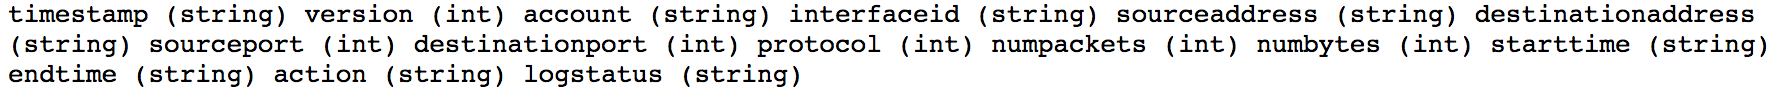
\includegraphics[width=3.5in]{./figures/561-default-format.png}}
%{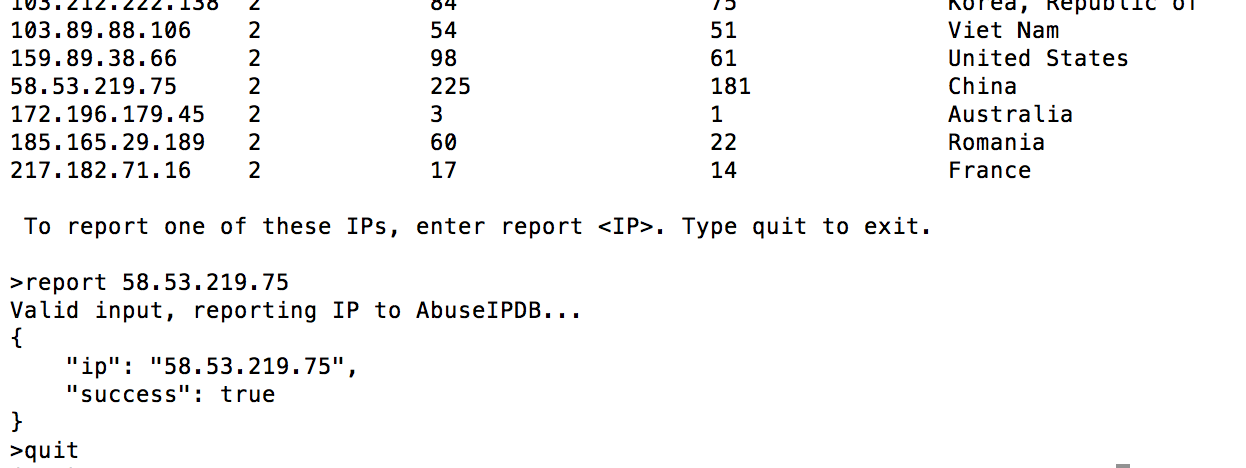
\includegraphics{./figures/561-irpSSHa-prompt.png}}
\caption{\small{Default input format}}
\label{fig:input-format}
\end{figure}

\begin{figure}[h]
%\resizebox{\textwidth}{!}
{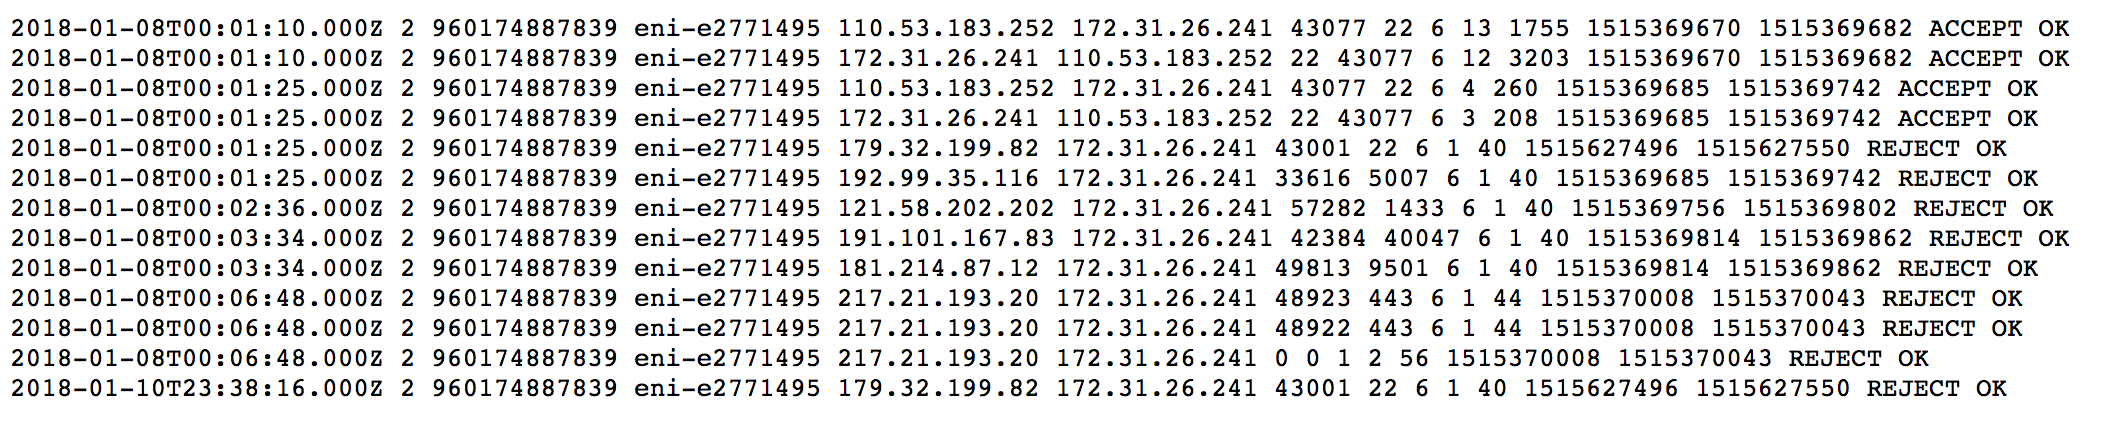
\includegraphics[width=4in]{./figures/561-sample-input.png}}
%{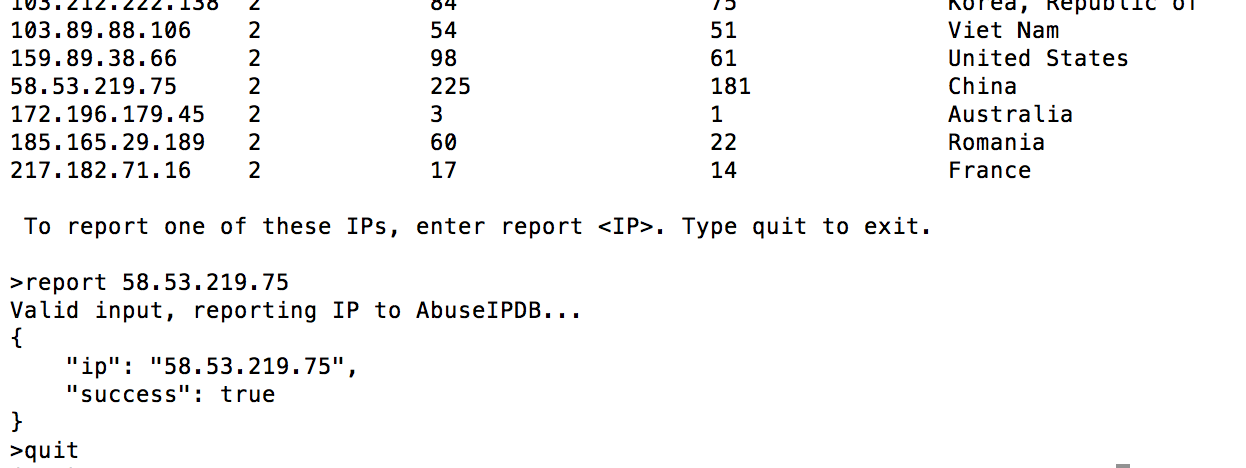
\includegraphics{./figures/561-irpSSHa-prompt.png}}
\caption{\small{Example of valid input in default format}}
\label{fig:sample-input}
\end{figure}

\begin{figure}[H]
%\resizebox{\textwidth}{!}
{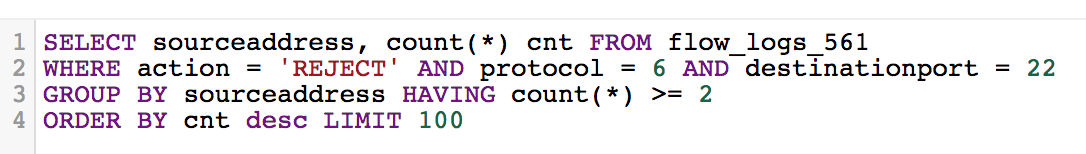
\includegraphics[width=3in]{./figures/561-athena-query.png}}
%{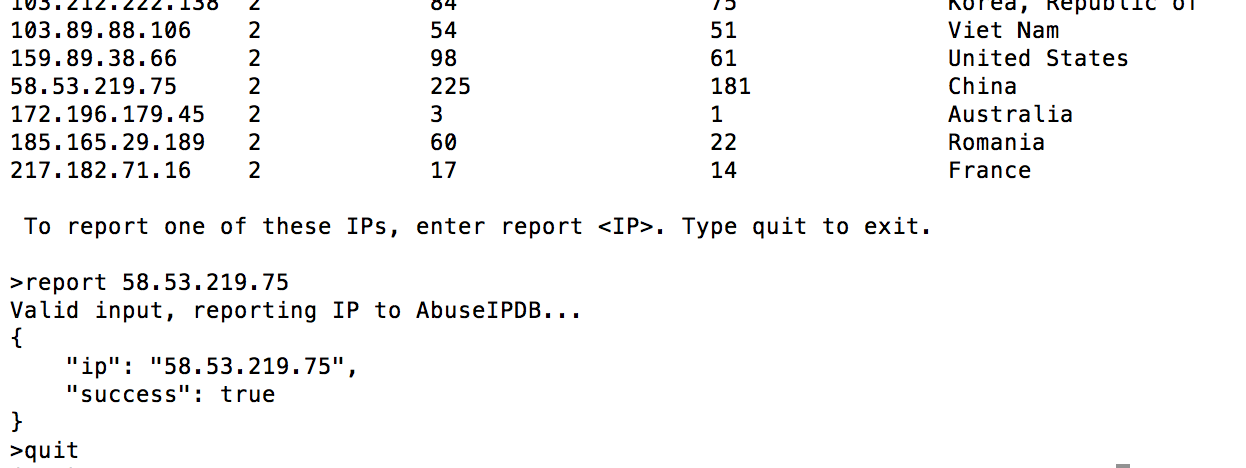
\includegraphics{./figures/561-irpSSHa-prompt.png}}
\caption{\small{Default SQL query used to identify potential attackers}}
\label{fig:query}
\end{figure}

After this information is obtained from the API for all IPs returned by the Athena query, the findings are presented to the user, along with an interactive prompt on the command line as shown in Figure~\ref{fig:prompt}. The user then has the option to review the results and select which, if any, of the source IPs to report. Entering \texttt{report <source IP>} with one of the IPs from the output will submit a report to AbuseIPDB via an HTTP POST. The report is submitted with the default or custom comment and is automatically tagged with categories "SSH" and "Brute Force". The report is then immediately viewable on the AbuseIPDB site, as shown in Figure~\ref{fig:report}.

\subsection{Additional Requirements}

It is recommended that the destination hosts for the input flows be secured enough to reject
unauthorized SSH traffic. In particular, ssh login should require public-key authentication and only whitelisted IPs should be allowed on the port running SSH, as discussed in Section 1.

\begin{figure}[H]
%\resizebox{\textwidth}{!}
{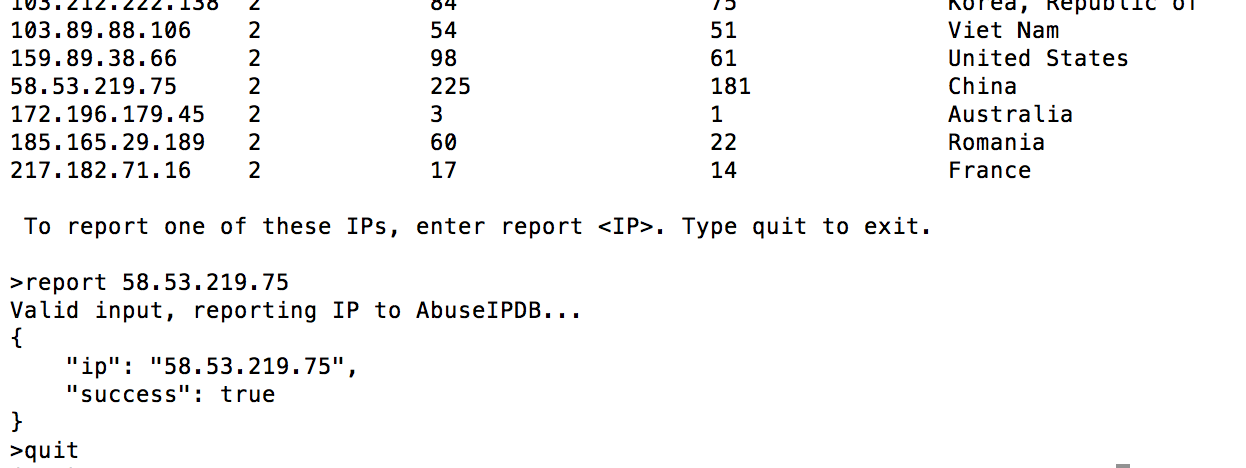
\includegraphics[width=3in]{./figures/561-irpSSHa-prompt.png}}
%{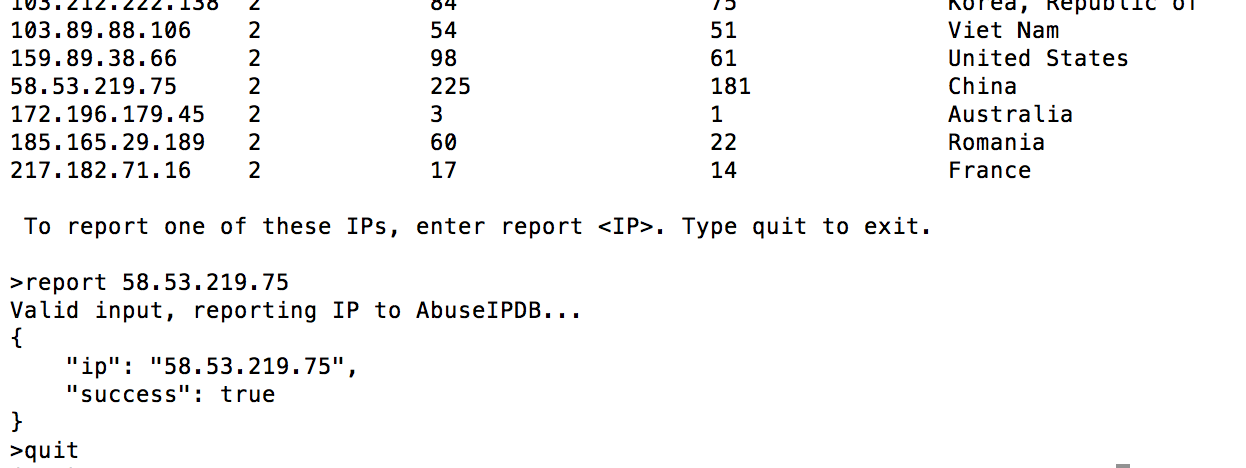
\includegraphics{./figures/561-irpSSHa-prompt.png}}
\caption{\small{Example command prompt interaction}}
\label{fig:prompt}
\end{figure}

\begin{figure}[H]
%\resizebox{\textwidth}{!}
{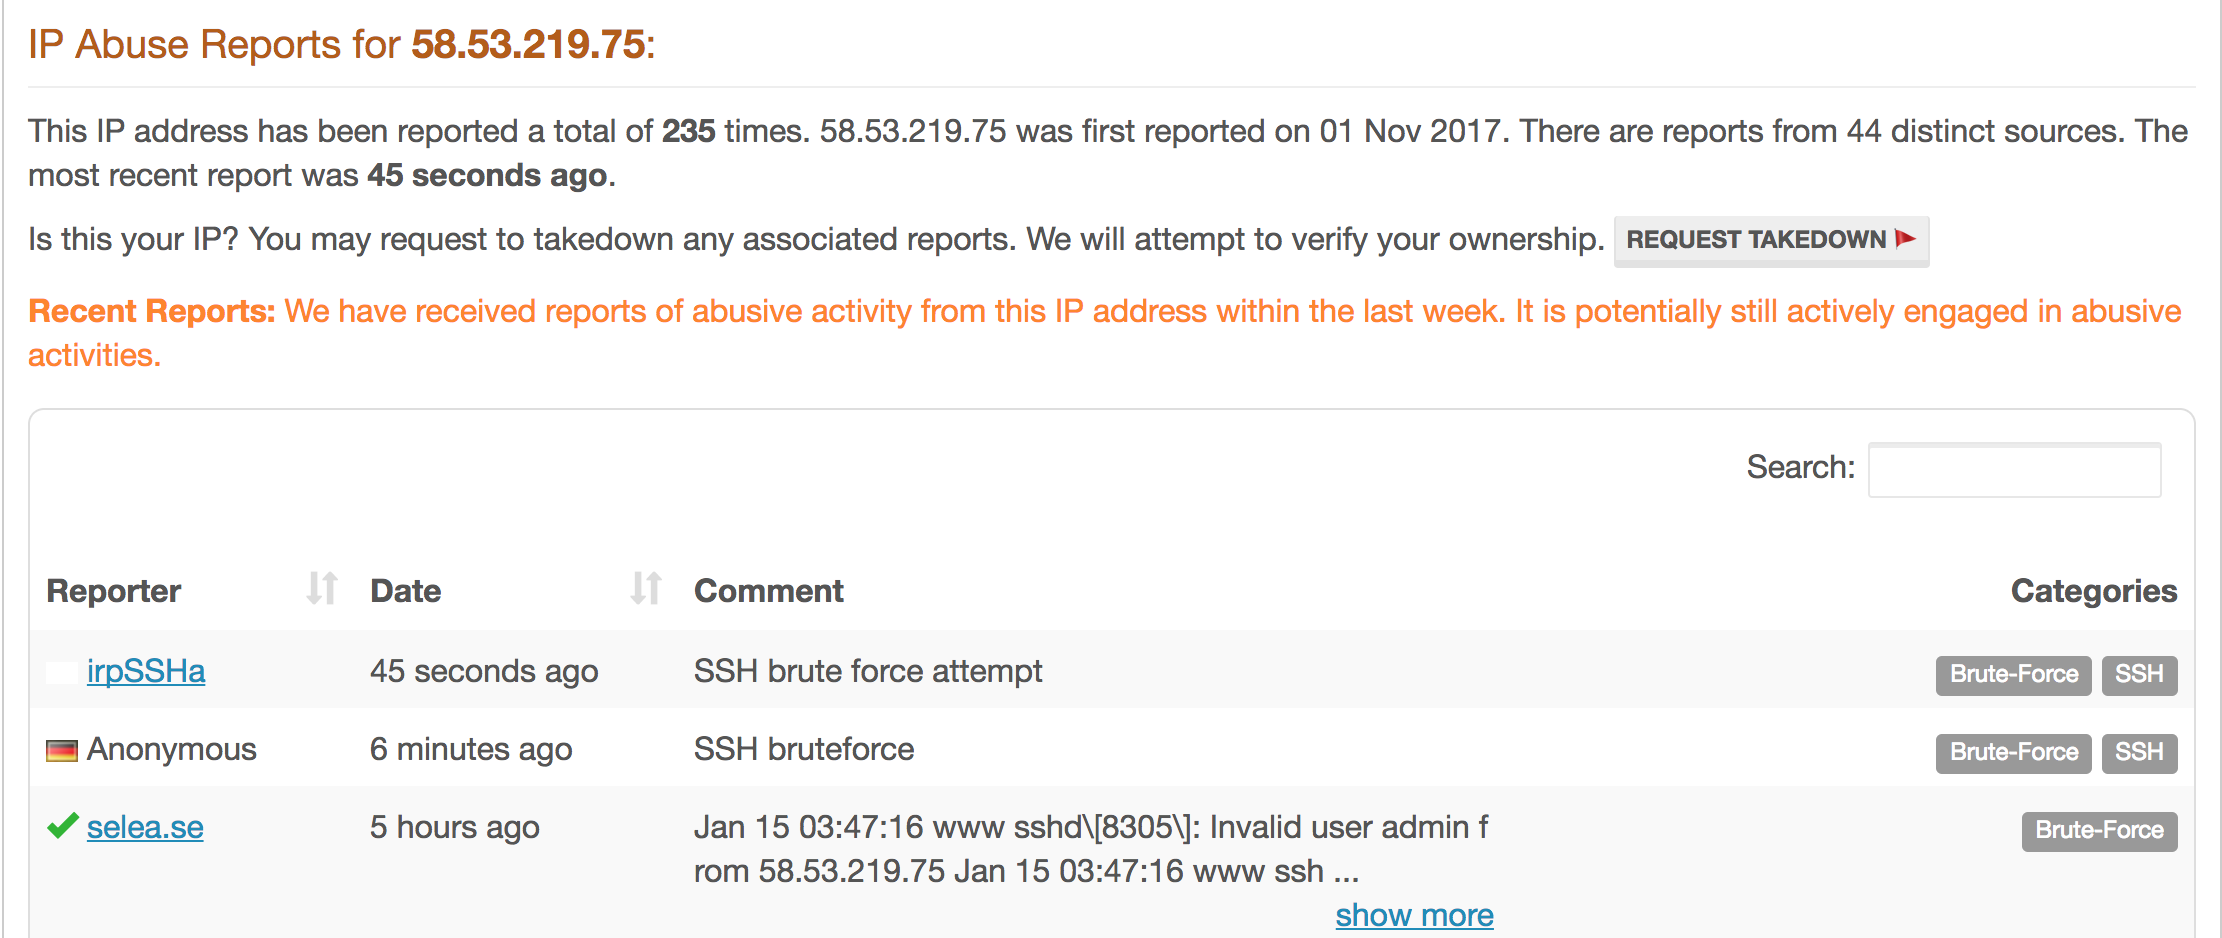
\includegraphics[width=3in]{./figures/561-AbuseIPDB-report.png}}
%{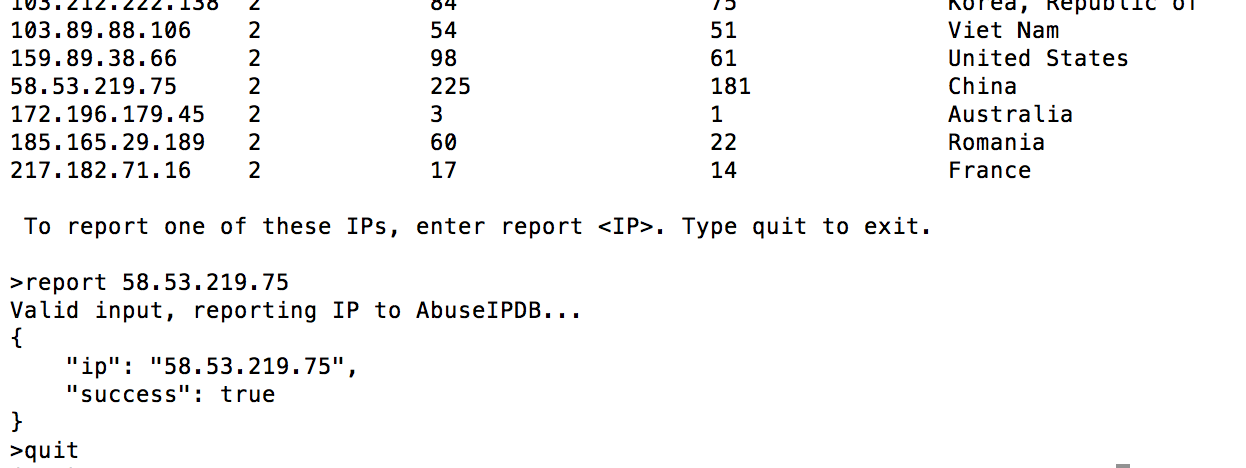
\includegraphics{./figures/561-irpSSHa-prompt.png}}
\caption{\small{Auto-generated report from irpSSHa on AbuseIPDB site}}
\label{fig:report}
\end{figure}

\subsection{Source Code}

The irpSSHa source code is available on GitHub:  \href{https://github.com/jlouthan/irpSSHa}{https://github.com/jlouthan/irpSSHa}.
\label{sec:design}






\subsection{Service Integrations}

irpSSHa is designed to be as simple as possible, while still providing users the ability to query large datasets, i.e., flow logs containing thousands or millions of records, efficiently, as well as the option of storing the logs and query results securely in the cloud for future reference. This is achieved by integrating with the services Amazon Simple Secure Storage (S3) and Amazon Athena, both products offered by Amazon Web Services (AWS). S3 stores objects consisting of files and metadata in online storage containers called buckets that offer fine-grained access control rules. Athena is a service that allows running standard SQL queries against formatted data stored in S3; Athena is serverless and scales automatically to ensure ad-hoc queries remain performant regardless of dataset size. Integrating with these services means that users of irpSSHa must be able to provide valid AWS credentials for an account with access to both S3 and Athena. This restriction is acknowledged as a tradeoff for the performance, reliability, and ease of querying and storing large amounts of data that the services bring to irpSSHa. Future work could involve exploring ways to evolve irpSSHa to have fewer or no third party dependencies.

As necessitated by the automatic abusive IP reporting functionality in irpSSHa, the tool also integrates with the AbuseIPDB API. In addition to reporting IPs, irpSSHa queries AbuseIPDB for data on file about IPs identified as potential attackers from the input data in order to corroborate suspicions that a given IP is engaging in an SSH brute force attack. Using a free account with AbuseIPDB incurs a rate limit of 1000 requests per day, so future extended work would require an account tier upgrade.

\begin{figure}[h]
%\resizebox{\textwidth}{!}
{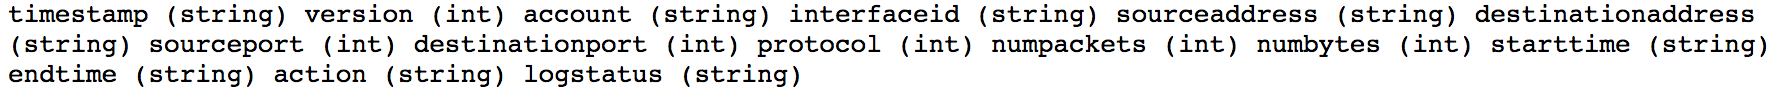
\includegraphics[width=3.5in]{./figures/561-default-format.png}}
%{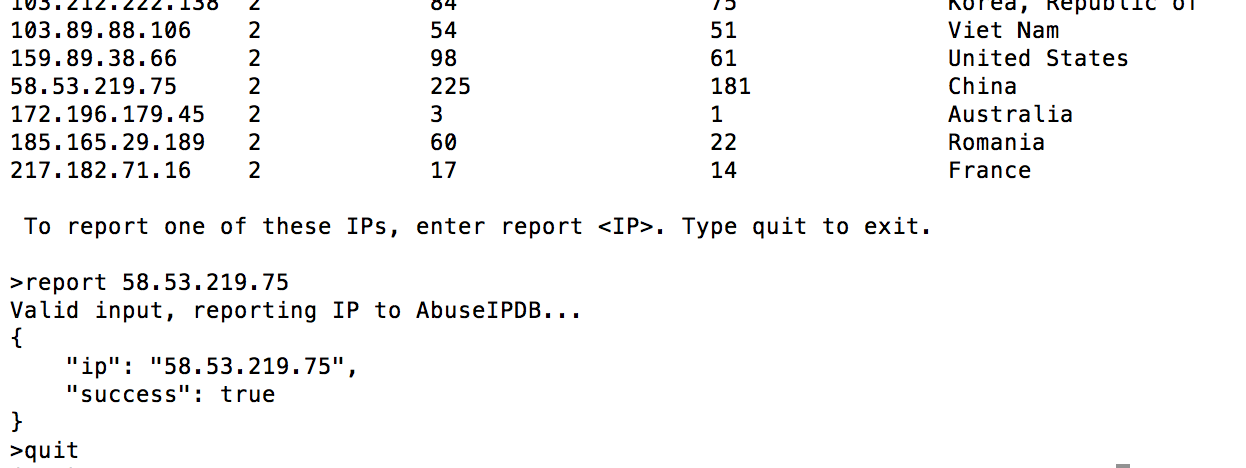
\includegraphics{./figures/561-irpSSHa-prompt.png}}
\caption{\small{Default input format}}
\label{fig:input-format}
\end{figure}

\begin{figure}[h]
%\resizebox{\textwidth}{!}
{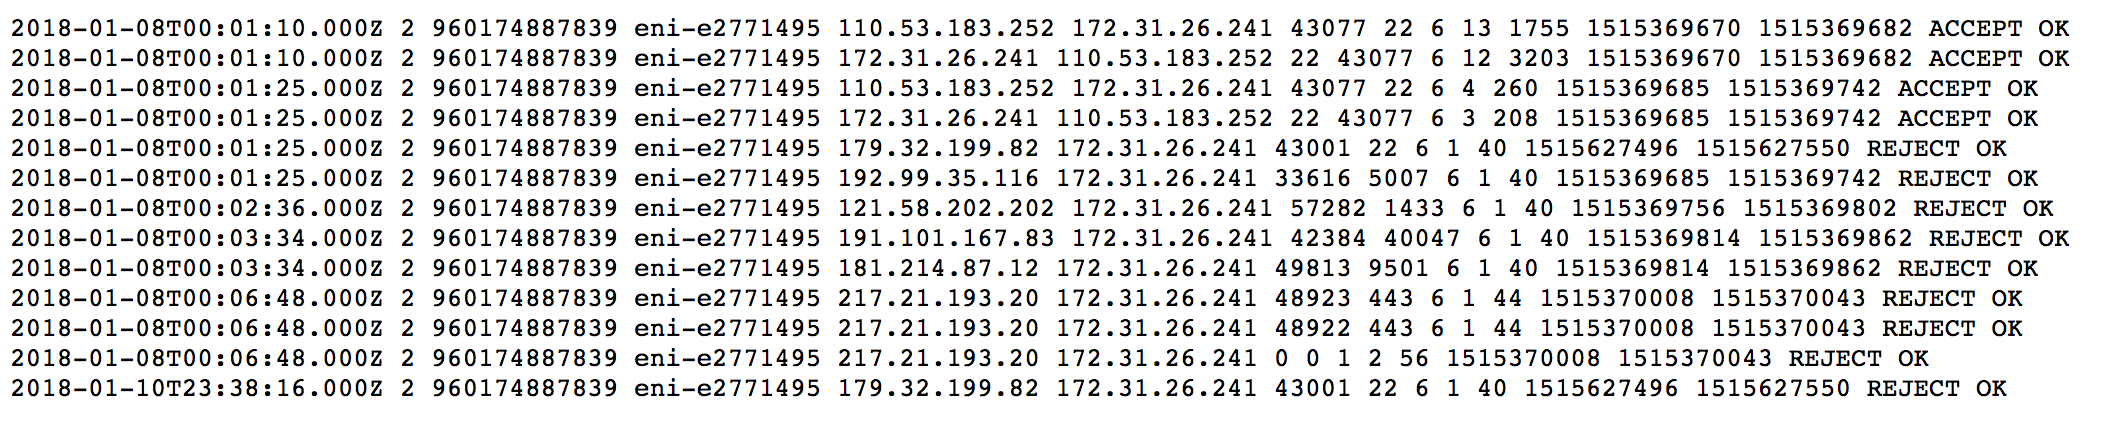
\includegraphics[width=4in]{./figures/561-sample-input.png}}
%{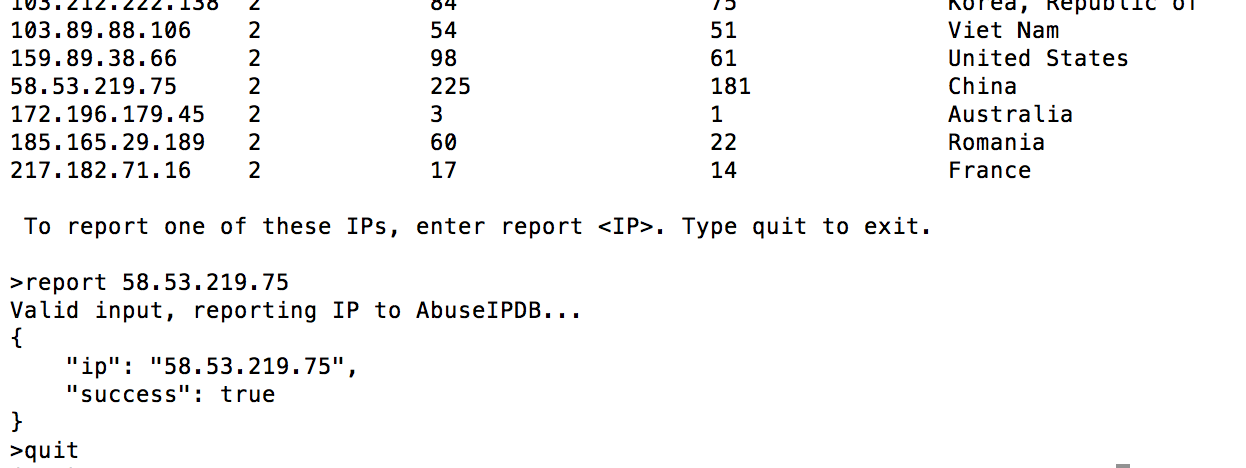
\includegraphics{./figures/561-irpSSHa-prompt.png}}
\caption{\small{Example of valid input in default format}}
\label{fig:sample-input}
\end{figure}

\subsection{Input Requirements}

IP flow logs are required as input to irpSSHa in order to report on attackers. Because SSH uses TCP, logs containing only TCP flows would be sufficient. To simplify the tool, rather than reading streams of data at the packet resolution, irpSSHa requires packets to be aggregated into flows prior to running the analysis. Output generated from existing tools like NetFlow [CITE?] and AWS VPC Flow Logs can be used as input, or individual packet traffic could be preprocessed before running irpSSHa. The format of the input must match the expected format of tool in order to run ad-hoc SQL queries as needed. The default format is modeled after the output from VPC Flow Logs and can be seen in Figure~\ref{fig:input-format}. Sample input adhering to this format can be seen in Figure~\ref{fig:sample-input}. The current format may appear a bit verbose; however, changing the format to match flow input data from different sources requires only a trivial change to the \texttt{create\_table} method in \texttt{athena\_helper.py}. More sample input files can be found in the GitHub repository. 

\begin{figure}[h]
%\resizebox{\textwidth}{!}
{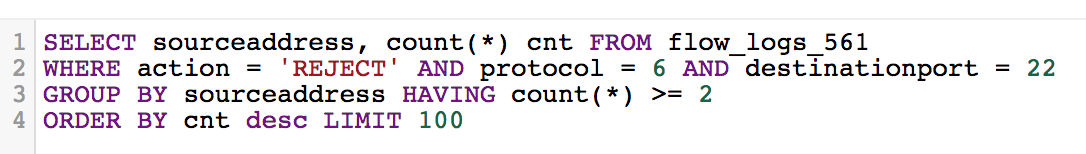
\includegraphics[width=3in]{./figures/561-athena-query.png}}
%{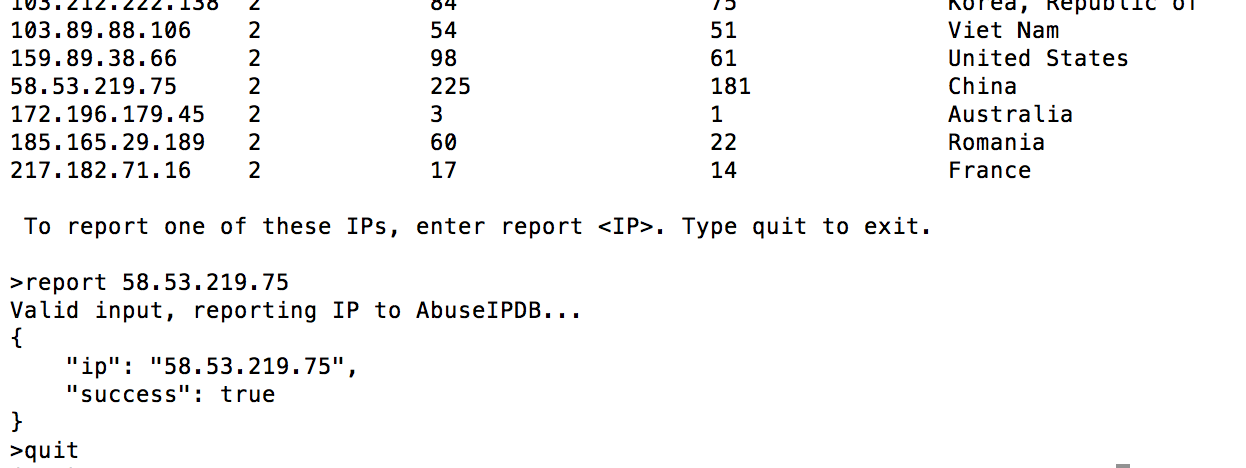
\includegraphics{./figures/561-irpSSHa-prompt.png}}
\caption{\small{Default SQL query used to identify potential attackers}}
\label{fig:query}
\end{figure}

\subsection{Detailed Implementation}

irpSSHa is written in Python and relies on the AWS SDK for Python, boto3, and the requests module for its service integrations. 

The tool begins execution by uploading the input file to S3. This involves creating a bucket for the irpSSHa data if it does not exist yet, and uploading the input to a new uniquely named folder. Next, a database is created in Athena if one for irpSSHa does not exist, and then a table is created in the database with the default or supplied field format. This table automatically imports the data from the appropriate bucket and folder in S3. At this point, the flow logs can be queried with standard SQL. irpSSHa executes the query in Figure~\ref{fig:query} to obtain a list of potential threats.

\begin{figure}[h]
%\resizebox{\textwidth}{!}
{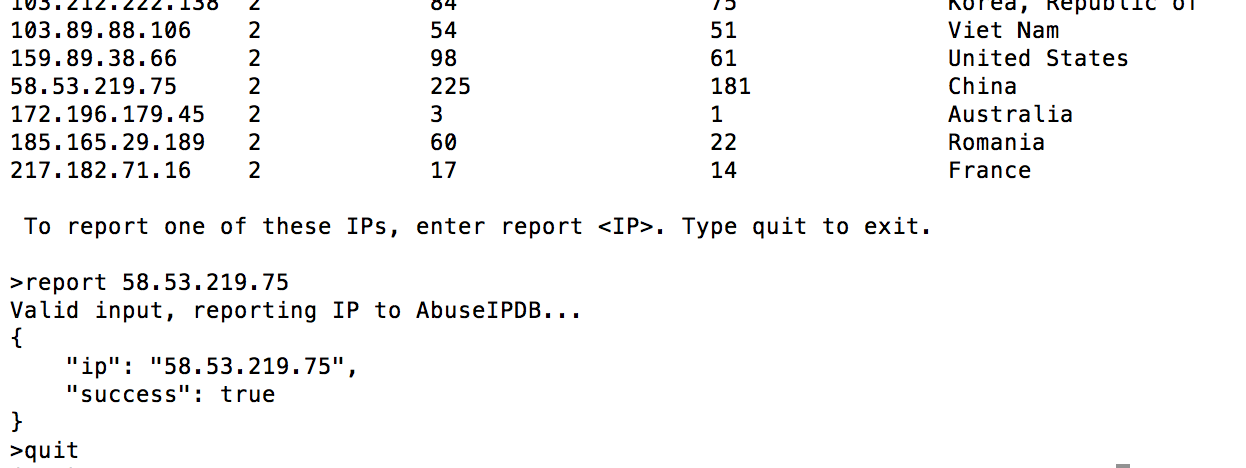
\includegraphics[width=3in]{./figures/561-irpSSHa-prompt.png}}
%{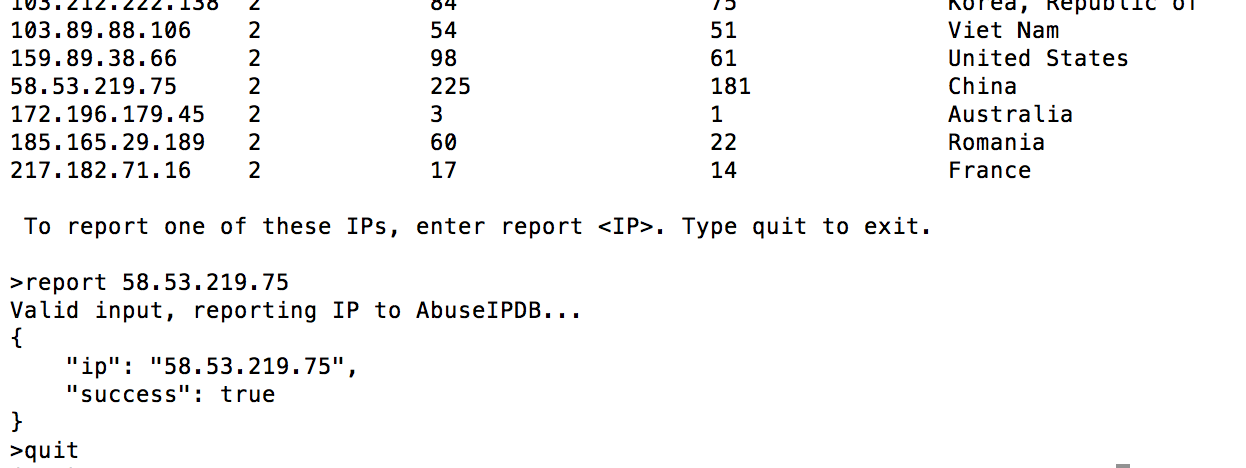
\includegraphics{./figures/561-irpSSHa-prompt.png}}
\caption{\small{Example command prompt interaction}}
\label{fig:prompt}
\end{figure}

\begin{figure}[h]
%\resizebox{\textwidth}{!}
{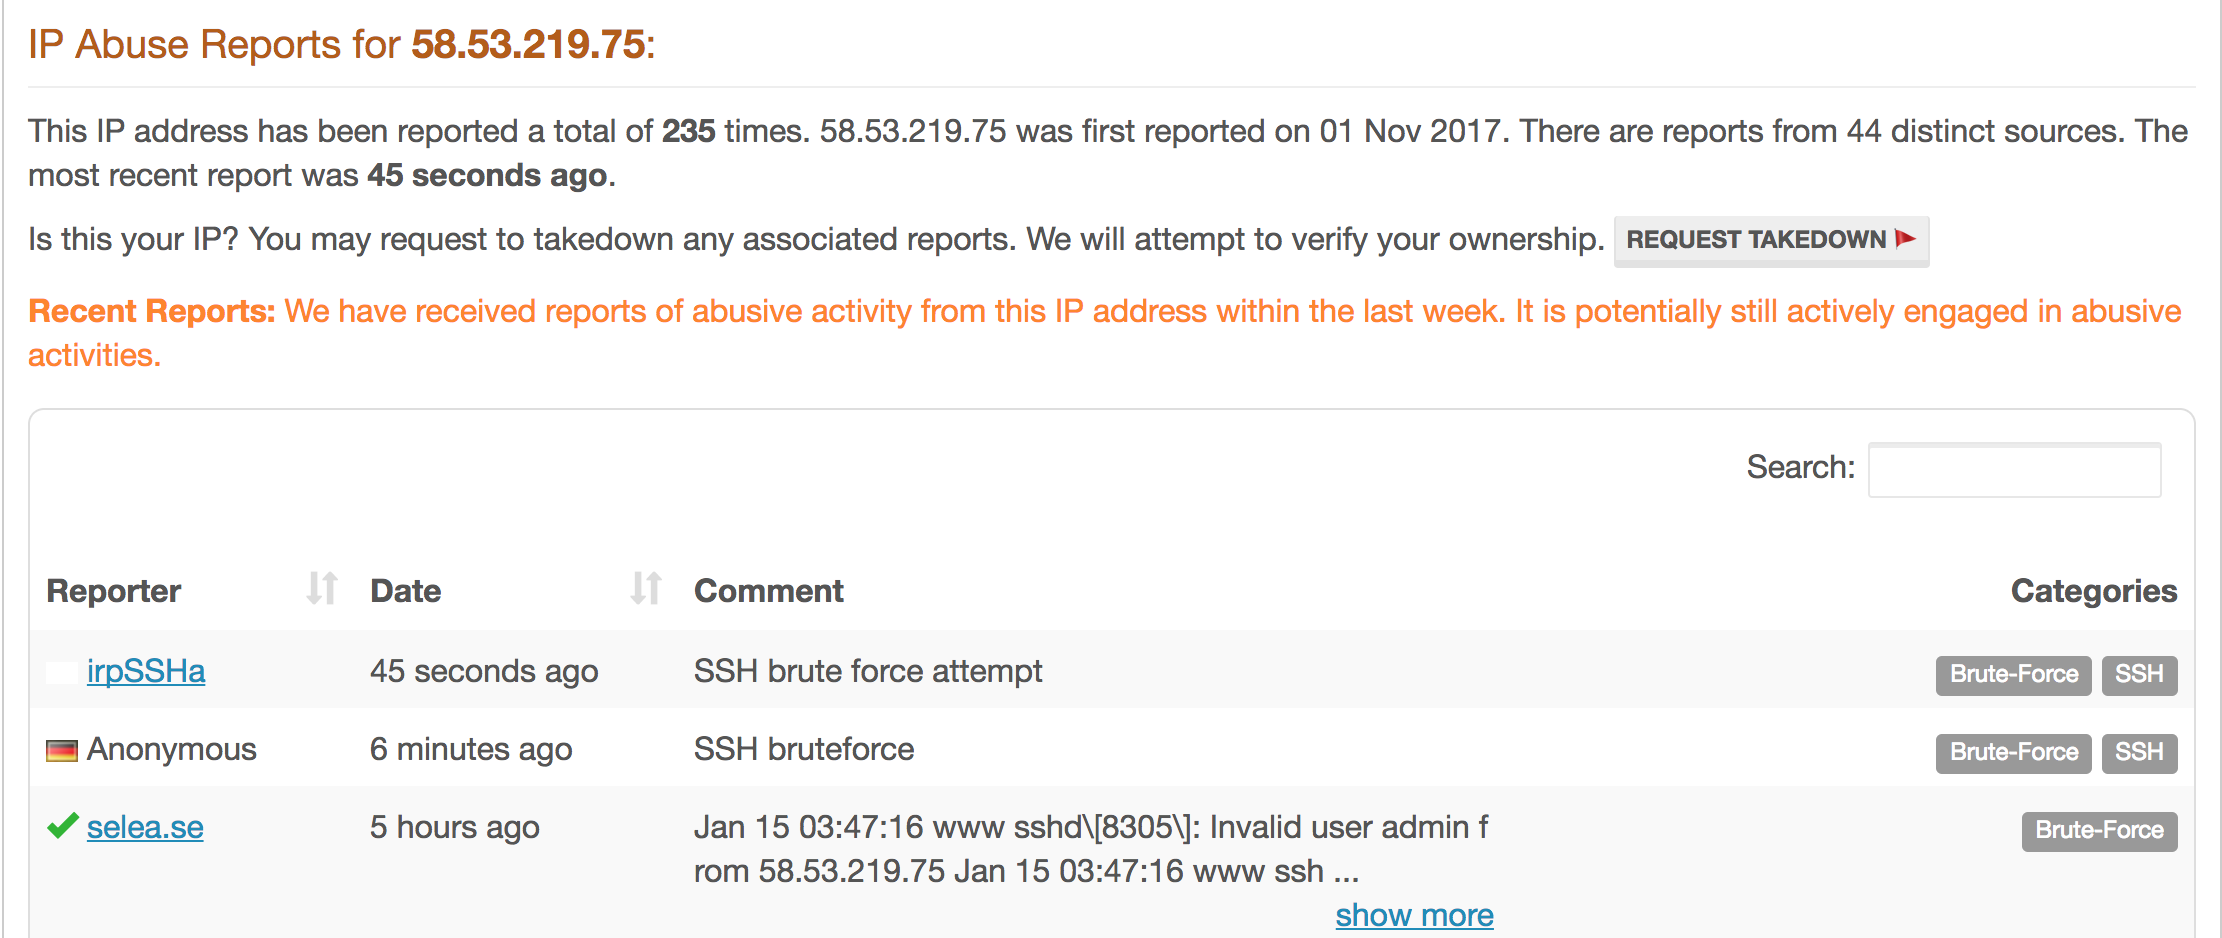
\includegraphics[width=3in]{./figures/561-AbuseIPDB-report.png}}
%{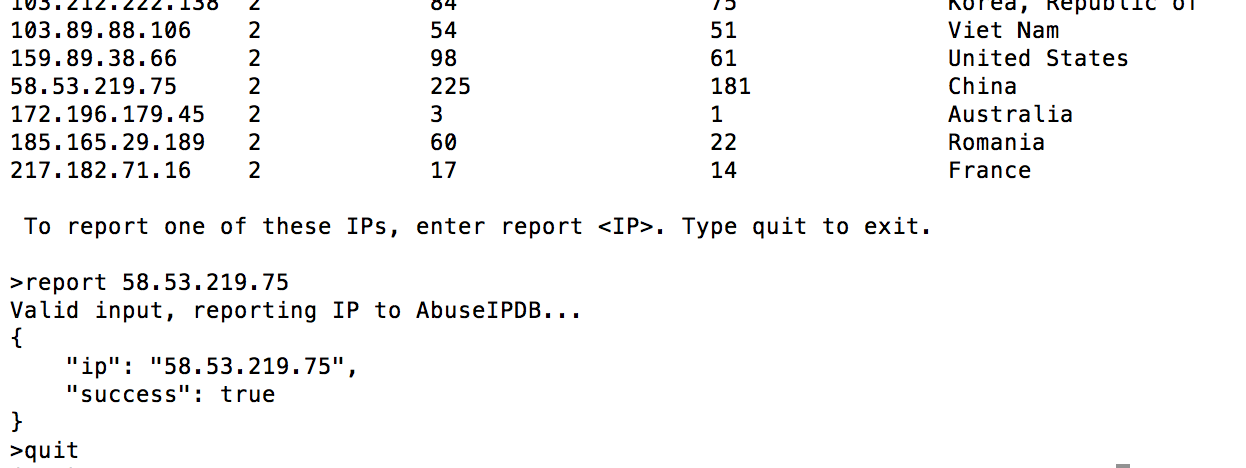
\includegraphics{./figures/561-irpSSHa-prompt.png}}
\caption{\small{Auto-generated report from irpSSHa on AbuseIPDB site}}
\label{fig:report}
\end{figure}

Once these IPs are identified by the query, irpSSHa issues a GET request to the AbuseIPDB API for each one and records the number of times it has been reported for abusive activity in the past 60 days, as well as the number of those reports that implicated the IP in attacks with the "SSH" or "Brute Force" label, or both. After this information is obtained from the API for all IPs returned by the query, the findings are presented to the user, along with an interactive prompt on the command line as in Figure~\ref{fig:prompt}. The user then has the option to review the results and select which, if any, of the source IPs to report. Entering \texttt{report <source IP>} with one of the IPs from the output will submit a report to AbuseIPDB via an HTTP POST. The report is submitted with the default or custom comment and is automatically tagged with categories "SSH" and "Brute Force". The report is then immediately viewable on the AbuseIPDB site, see Figure~\ref{fig:report}.

\subsection{Additional Requirements}

It is recommended that the destination hosts for the input flows be secured enough to reject
unauthorized SSH traffic. In particular, ssh login with username/password should be disabled and only whitelisted IPs should be allowed, as discussed in section [SECTION 1 REFERENCE].

\subsection{Source Code}

The irpSSHa source code is available on GitHub:  \href{https://github.com/jlouthan/irpSSHa}{https://github.com/jlouthan/irpSSHa}.

\section{Evaluation}
\label{sec:eval}



\begin{figure}[h]
%\resizebox{\textwidth}{!}
{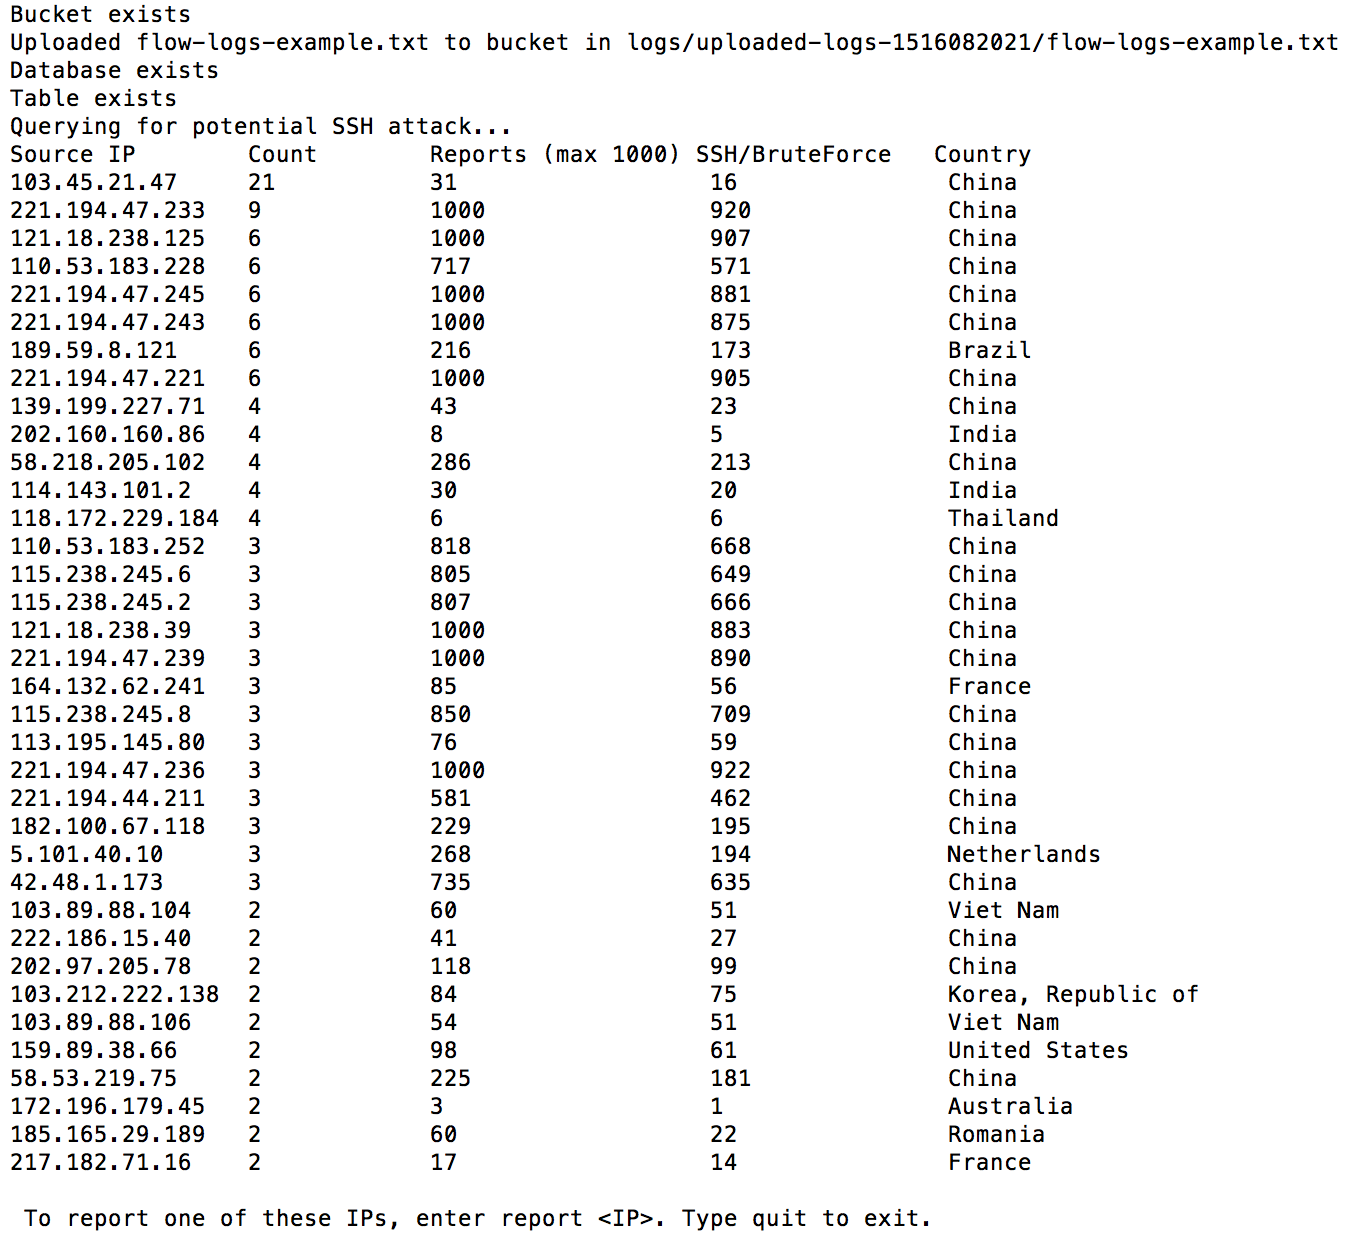
\includegraphics[width=3in]{./figures/561-irpSSHa-output-1.png}}
%{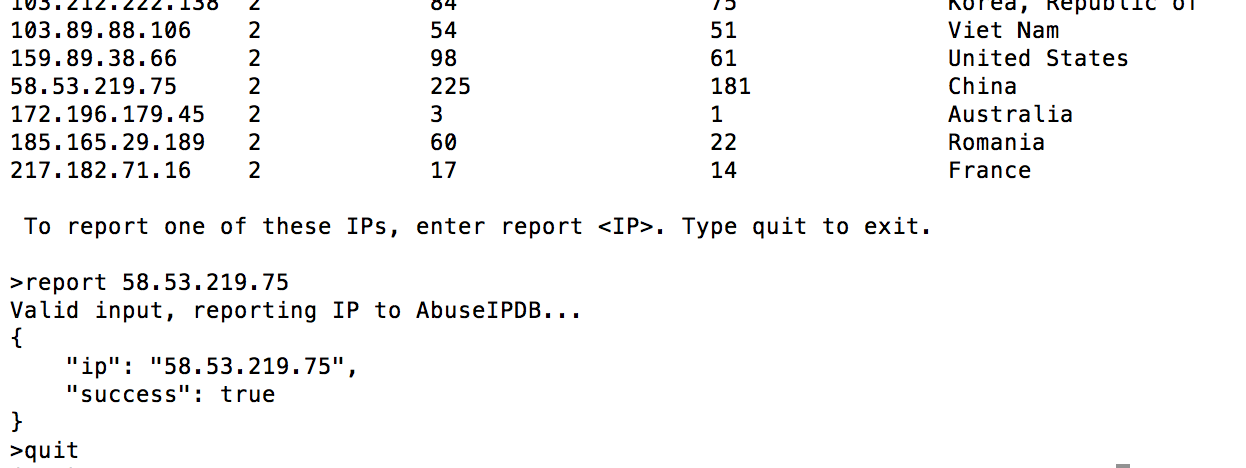
\includegraphics{./figures/561-irpSSHa-prompt.png}}
\caption{\small{Output from running irpSSHa with the first example IP flow dataset}}
\label{fig:output1}
\end{figure}

\begin{figure}[h]
%\resizebox{\textwidth}{!}
{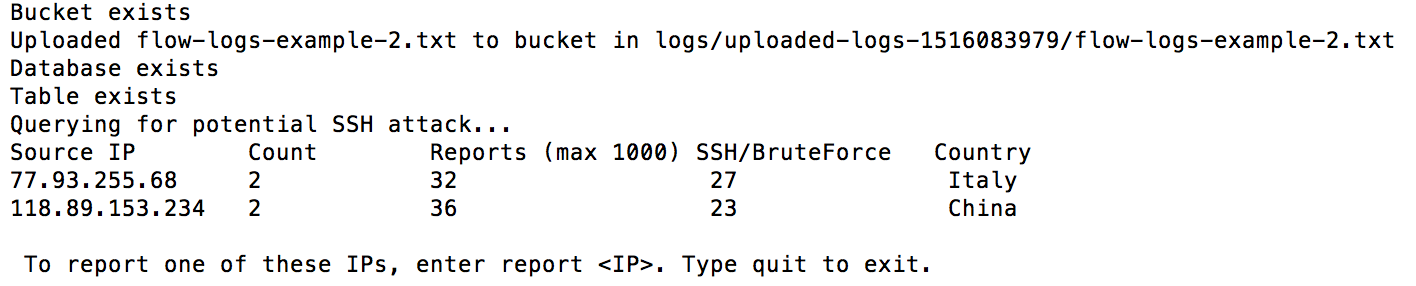
\includegraphics[width=3in]{./figures/561-irpSSHa-output-2.png}}
%{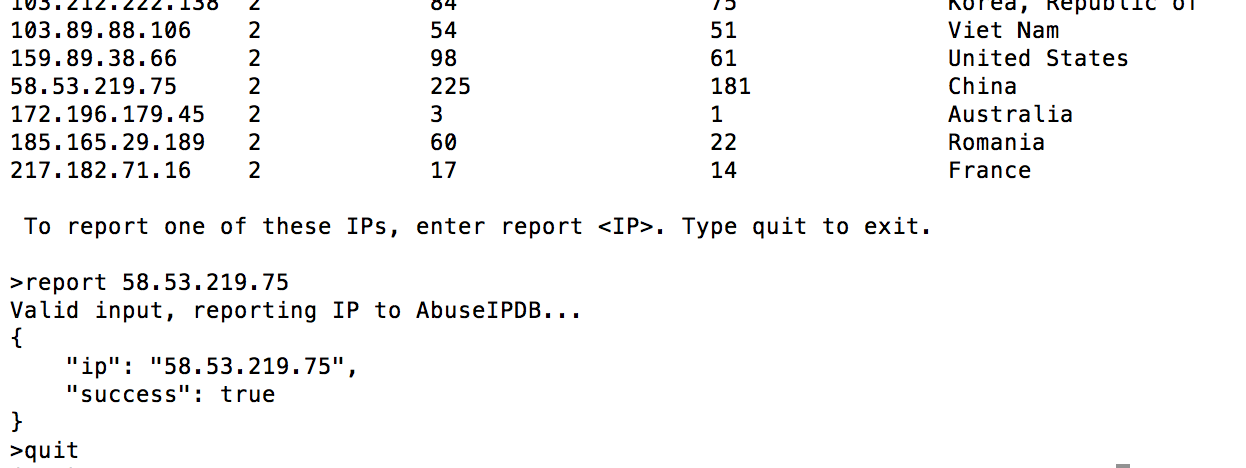
\includegraphics{./figures/561-irpSSHa-prompt.png}}
\caption{\small{Output from running irpSSHa with the second example IP flow dataset}}
\label{fig:output2}
\end{figure}

To evaluate irpSSHa, two IP flow log datasets were used as input. The flow logs were collected from VPC Flow Logs monitoring on an AWS EC2 t1.micro instance running Ubuntu 14.04 in the US East (N. Virginia) region. The first input dataset spanned a time period of four days, from midnight GMT on January 8th, 2018, to midnight GMT on January 12th, 2018. The second spanned a time period of four hours, from 1:00am GMT on January 15th, 2018, to 5:00am GMT on January 15th, 2018. The datasets included 13058 and 476 flow records, respectively. The irpSSHa output for each can be seen in Figure~\ref{fig:output1} and Figure~\ref{fig:output2}

The output is separated into five columns. The Source IP column contains distinct IPs that were identified as potential SSH brute force attackers within the input flows. The Count column contains the number of flows in the input that contained unauthorized SSH access attempts from the IP. The Reports column indicates how many times in the past 60 days the source IP has been reported to AbuseIPDB. A limitation of the AbuseIPDB API is that the maximum value returned for this field is 1000, so source IPs with 1000 reports in the output were very likely reported a significant number of times \textit{more} than 1000. The data in the fourth column represents the number of the reports that indicated the IP was suspected of an SSH attack, brute force attack, or both. The last column contains the name of the country in which the source IP originates.

As seen in the output, the smaller dataset indicated two IPs potentially involved in SSH brute force attack attempts. In both executions of irpSSHa, the minimum threshold for observing unauthorized SSH access attempts was two flows. Each IP in the smaller input's results was reported to AbuseIPDB at least 30 times within the last 60 days, with the majority of each implicating the IP in SSH and/or brute force attacks. The output for the larger dataset identifies 36 different source IPs as potential attackers, with 8 of them having been reported at least 1000 times within the last 60 days to AbuseIPDB. The potential attackers were responsible for a total of 145 unauthorized SSH access attempts (the sum of the Count column). If we decrease the minimum threshold from two to one, AbuseIPDB rate limits are quickly exceeded, but 101 more IPs are identified from the larger dataset, bringing the total up to 246 potential brute force attack attempts in four days. While not quite as large as some reports using dedicated honeypots, these numbers are consistent with what would be expected. In addition, we observe that, of the 36 source IPs in the larger input's table, 23 or about 64\% of them originate in China.

\section{Related Work}
Full featured intrusion detection systems (IDSs) such as Snort~\cite{snort} and Bro~\cite{bro} can run real time packet analysis on an end host with filters to implicate traffic in potential SSH brute force attacks. Adding the ability to run queries on traffic in real time is included in the scope of future work for irpSSHa. However, for use cases where historical traffic data from any host needs to be analyzed for attacks and reported upon, irpSSHa would be ideal over complex IDS systems running on destination hosts.

The network telemetry system Sonata~\cite{sonata} offers a query interface to allow administrators performant access to traffic analytics that could feasibly be used to identify potential SSH attackers in a similar manner as irpSSHa's Athena queries. However, Sonata does not run on the end host, and a reporting mechanism would need to be added on top of Sonata to add abusive IPs to a blacklist. 

Several smaller services providing intrusion prevention are perhaps the most comparable to irpSSHa in goals and functionality. These services, including tools like DenyHosts~\cite{denyhosts}, sshguard~\cite{sshguard}, and the popular Fail2Ban~\cite{fail2ban}, scan log files on the end host for signs of malicious activity and block IPs of repeat offenders. Some have configuration options for reporting attacker IPs to a system administrator. The main goals of these tools is to secure the host on which they are running; this is in contrast to irpSSHa, which aims primarily to identify abusive IPs for the purpose of sharing with reputable public blacklists.
\label{sec:related}



Full featured intrusion detection systems (IDSs) such as Snort~\cite{snort} and Bro~\cite{bro} can run real time packet analysis on an end host with filters to implicate traffic in potential SSH brute force attacks. Adding the ability to run queries on traffic in real time is included in the scope of future work for irpSSHa. However, for use cases where historical traffic data from any host needs to be analyzed for attacks and reported upon, irpSSHa would be ideal over complex IDS systems running on destination hosts.

The network telemetry system Sonata~\cite{sonata} offers a query interface to allow administrators performant access to traffic analytics that could feasibly be used to identify potential SSH attackers in a similar manner as irpSSHa's Athena queries. However, Sonata does not run on the end host, and a reporting mechanism would need to be added on top of Sonata to add abusive IPs to a blacklist. 

Several smaller services providing intrusion prevention are perhaps the most comparable to irpSSHa in goals and functionality. These services, including tools like DenyHosts~\cite{denyhosts}, sshguard~\cite{sshguard}, and the popular Fail2Ban~\cite{fail2ban}, scan log files on the end host for signs of malicious activity and block IPs of repeat offenders. Some have configuration options for reporting attacker IPs to a system administrator. The main goals of these tools is to secure the host on which they are running; this is in contrast to irpSSHa, which aims primarily to identify abusive IPs for the purpose of sharing with reputable public blacklists.

\section{Conclusions}
\label{sec:conclusion}





%% Bibliography
%\vspace{-1ex}
%\linespread{1.0}
%\setlength{\bibsep}{1pt}
%\footnotesize
\small
\bibliography{local}
\bibliographystyle{abbrvnat}
\begin{thebibliography}{9}
\bibitem{sshbook} 
Daniel J. Barrett and Richard E. Silverman. 
\textit{The Secure Shell: The Definitive Guide}. 
O'Reilly Associates, Inc, Sebastopol, CA, 2011.
\\\texttt{https://docstore.mik.ua/orelly/networking\_2ndEd/ssh/copyrght.htm}
 
\bibitem{stealthy} 
Mobin Javed and Vern Paxson.
Detecting Stealthy, Distributed SSH Brute-Forcing.
in \textit{ACM CCS}. 
2013.
%[\textit{On the electrodynamics of moving bodies}]. 
%Annalen der Physik, 322(10):891�921, 1905.
 
\bibitem{symantec} 
Christian Seifert.
Analyzing Malicious SSH Login Attempts.
\\\texttt{https://www.symantec.com/connect/articles/analyzing-malicious-ssh-login-attempts}

\bibitem{sucuri1} 
Daniel Cid.
SSH Brute Force -- The 10 Year Old Attack That Still Persists.
\\\texttt{https://blog.sucuri.net/2013/07/ssh-brute-force-the-10-year-old-attack-that-still-persists.html}

\bibitem{sucuri2} 
Daniel Cid.
SSH Brute Force Compromises Leading to DDoS.
\\\texttt{https://blog.sucuri.net/2016/09/ssh-brute-force-compromises-leading-to-ddos.html}

\bibitem{abuse} 
AbuseIPDB.
\\\texttt{https://www.abuseipdb.com/}

\bibitem{snort} 
Snort.
\\\texttt{https://www.snort.org/}

\bibitem{bro} 
Bro.
\\\texttt{https://www.bro.org/}

\bibitem{denyhosts} 
Deny Hosts.
\\\texttt{http://denyhosts.sourceforge.net/}

\bibitem{sshguard} 
sshguard.
\\\texttt{https://www.sshguard.net/}

\bibitem{fail2ban} 
Fail2Ban.
\\\texttt{https://www.fail2ban.org}

\bibitem{sonata} 
Arpit Gupta, Rob Harrison, Ankita Pawar, Marco Canini,
Nick Feamster, Jennifer Rexford, Walter Willinger.
Sonata: Query-Driven Streaming Network Telemetry.
2017.

\end{thebibliography}

\end{document}

